\section{Alhazenov problem}

Spoznajmo zanimiv problem, ki izhaja že iz stare Grčije. Čez poglavje si bomo pogledali več njegovih različic in poskusili najti origami konstrukcijo njegove rešitve.

\subsubsection*{Starogrški izvor problema}

V osnovi gre za problem s področja optike, ki naj bi ga zastavil grški matematik Ptolemaj (prb.\ 85--170 po Kr.): \emph{Pri danem sferičnem zrcalu in viru svetlobnega žarka poišči točko na zrcalu, od katere se bo svetlobni žarek odbil v oko opazovalca} (slika~\ref{fig:ptolemaj}).

\begin{figure}[h]
    \centering
    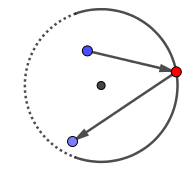
\includegraphics[width=0.25\textwidth]{images/alhazen/ptolemajev_problem.png}
    \caption[Ptolemajev problem]{Ptolemajev optični problem.}
    \label{fig:ptolemaj}
\end{figure}

Rešitev se da preformulirati v iskanje točke na krožnici, v kateri polmer krožnice razpolavlja kot, ki ga opravi svetlobni žarek. To velja zaradi \emph{odbojnega zakona}, vendar tega v takratni Grčiji še niso poznali. Pojdimo na začetek in opazujmo, kako se je oblika Ptolemajevega problema spreminjala skozi čas.

Grški matematik Heron iz Aleksandrije, med drugim znan po svoji Heronovi formuli za izračun ploščine trikotnika z danimi dolžinami stranic, je okoli leta 100 po Kr.\ zastavil in rešil naslednje vprašanje, ki je različica Ptolemajevega problema: \emph{Na isti strani premice ležita točki $A$ in $B$. Poišči točko $C$ na premici, da bo pot od točke $A$ do $B$ preko točke $C$ najkrajša}\footnote{Predpostavimo evklidsko metriko.}.

Sam točko $C$ konstruira zelo enostavno -- najprej točko $B$ zrcali čez premico v točko $B'$, nato pa s točko $C$ označi presečišče premice in daljice $AB'$ (slika~\ref{fig:heron}). Ker velja $|CB| = |CB'|$, je $|AC| + |CB| = |AC| + |CB'| = |AB'|$. Dolžina $|AB'|$ najkrajša možna razdalja med točkama $A$ in $B'$, zato je točka $C$ rešitev vprašanja.

\begin{figure}[h]
    \centering
    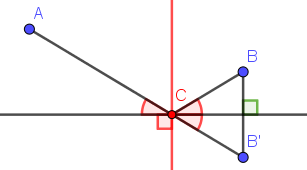
\includegraphics[width=0.4\textwidth]{images/alhazen/heron.png}
    \caption[Heronovo vprašanje]{Heronova konstrukcija najkrajše poti od točke $A$ do točke $B$.}
    \label{fig:heron}
\end{figure}

Zgornja konstrukcija pa je grškemu matematiku ponudila še nekaj -- opazil je, da pravokotnica na premico skozi točko $C$ namreč razpolavlja kot $\angle ACB$ (gl.\ rdeče oznake na sliki~\ref{fig:heron}). Tako lahko njegovo vprašanje preoblikujemo v: \emph{Na isti strani premice ležita točki $A$ in $B$. Poišči točko $C$ na premici, ki razpolavlja kot $\angle ACB$.}

\opomba{Bralec je prepuščen enostaven premislek, kako konstruirati točko $C$ z origamijem.}

\subsubsection*{Formulacija Alhazenovega problema}

S tem novim znanjem je Heron postavil temelje, na katerih je več stoletij kasneje matematik, astronom in fizik Ibn al-Haytham oz.\ po naše Alhazen (prb.\ 965--1040 na območju današnjega Iraka) formuliral odbojni zakon, ki pravi, da sta vpadni in odbojni kot žarka svetlobe od površja enaka. Alhazen se je tudi prvi bolj poglobil v Ptolemajev problem in prišel do pomembnih ugotovitev, zato problem ponekod imenujejo tudi Ptolemaj-Alhazenov problem\footnote{\emph{Ptolemy-Alhazen's problem}, op.\ prev.}, tu bomo uporabili imenovanje \emph{Alhazenov problem}\footnote{\emph{Alhazen's problem}, op.\ prev.}. 

Zopet formulirajmo problem. Namesto premice imamo torej krožnico $\mathcal{K}$ s središčem $O$. Naj točki $A$ in $B$ ležita znotraj krožnice (za točki zunaj krožnice je reševanje problema enako, je pa Alhazen originalno predpostavil ta položaj). Iščemo točko $C$ na krožnici $\mathcal{K}$, da se bo svetlobni žarek iz točke $A$ v točki $C$ odbil v točko $B$. Na enak način kot Hero lahko premislimo, da mora polmer $OC$ razpolavljati kot $ACB$ (slika~\ref{fig:alhazen1}).

\begin{figure}[h]
    \centering
    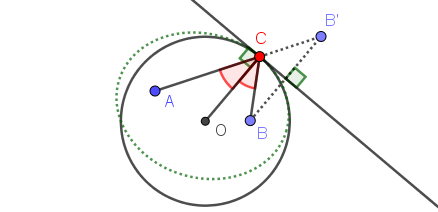
\includegraphics[width=0.6\textwidth]{images/alhazen/alhazen1.png}
    \caption[Alhazenov problem]{Ena od rešitev Alhazenovega problema v splošnem.}
    \label{fig:alhazen1}
\end{figure}

Za razliko od Heronove konstrukcije tu ne znamo konstruirati točke $B'$, saj je premica, čez katero bi morali zrcaliti točko $B$ (in tako s presečiščem daljice $AB'$ in premice dobiti točko $C$), ravno tangenta v točki $C$. Premice torej ne moremo dobiti brez točke $C$, točke $C$ pa ne moremo dobiti brez te premice. Tu se pokaže razsežnost problema.

Že tisoč let nazaj je Alhazen pokazal, da se da problem rešiti s stožnicami. V dolgem in za marsikaterega kasnejšega matematika zapletenem dokazu je pokazal, da so izkane točke odboja preseki te krožnice z določeno hiperbolo~\cite{wilk2015}. Algebraično rešitev je l.\ 1965 našel Jack M.\ Elkin, l.\ 1989 je problem rešil še Harald Riede, za njim l.\ 1997 pa še Peter M.\ Neumann. A pojdimo po vrsti.

\opomba{Opazimo lahko tudi, da ima zaradi enakega vpadnega in odbojnega kota žarka v točka $C$ lastnost točke, ki leži na \emph{elipsi} z goriščema $A$ in $B$ (na sliki~\ref{fig:alhazen1} označena s prekinjeno črto). Tangenta na krožnico v točki $C$ je hkrati tudi tangenta na elipso v isti točki, torej lahko problem preoblikujemo v iskanje vseh elips z goriščema v $A$ in $B$, ki so tangentne na krožnico $\mathcal{K}$. Vendar ne poznamo postopka, ki bi nam lahko poiskal enačbo te elipse, saj je ta odvisna od točke $C$, ta pa od tangente in obratno. Torej smo zopet na istem.}

\subsubsection*{Prevedba problema na reševanje kvartične enačbe}

Alhazen je med drugi ugotovil, da se da problem prevesti tudi v reševanje enačbe četrte stopnje. Naslednji nastavek za izpeljavo je vzeta iz~\cite[138--139]{geometricconstructions}. Brez škode za splošnost predpostavimo, da je krožnica $\mathcal{K}$ enotska, $O = (0,0), A = (0,a)$ in $B=(b,c)$ za take $0 \leq a, b, c \leq 1$, da te točke med sabo paroma ne sovpadajo (slika~\ref{fig:alhazen2}). Naj bo $C=(x,y)$ iskana točka na krožnici $\mathcal{K}$. Iz tega sledi pogoj
\begin{equation}
    \label{eq:pogoj_alh1}
    x^2 + y^2 = 1.
\end{equation}

\begin{figure}[h]
    \centering
    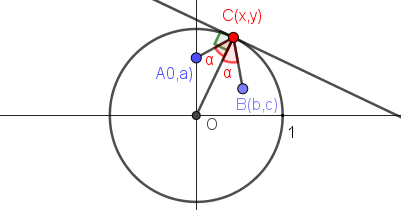
\includegraphics[width=0.6\textwidth]{images/alhazen/alhazen2.png}
    \caption[Alhazenov problem -- izpeljava]{Podlaga za izpeljavo kvartične enačbe za Alhazenov problem.}
    \label{fig:alhazen2}
\end{figure}

Naj bodo premice $AC$, $OC$ in $BC$ nosilke istoimenskih daljic in naj bo za vsako premico $i$ s $k_i$ označen njen koeficient. Dobimo
\begin{align*}
    &k_{AC} = \frac{y-a}{x}, \\
    &k_{OC} = \frac{y}{x}, \\
    &k_{BC} = \frac{y-c}{x-b}.
\end{align*}
Označimo $\alpha = \angle ACO = \angle OCB$. Ker sta kota enaka, velja
\begin{align*}
    \tan \alpha &= tan \alpha, \\
    \frac{k_{AC} - k_{OC}}{1 + k_{AC} k_{OC}} &= \frac{k_{OC} - k_{BC}}{1 + k_{OC} k_{BC}}, \\
    \frac{\frac{y-a}{x} - \frac{y}{x}}{1 + \frac{y-a}{x} \cdot \frac{y}{x}} &= \frac{\frac{y}{x} - \frac{y-c}{x-b}}{1 + \frac{y}{x} \cdot \frac{y-c}{x-b}}.
\end{align*}
Slednjo enačbo poenostavimo in z upoštevanjem pogoja~\ref{eq:pogoj_alh1} dobimo
$$ y(b + 2acx) = ab + (a+c)x - 2abx^2.$$
Enačbo kvadriramo, spet upoštevamo pogoj~\ref{eq:pogoj_alh1} in dobimo enačbo četrte stopnje (\textcolor{red}{si poračunala, tudi z wolframom, je na enem listu}):
$$ 4a^2(b^2 + c^2)x^4 - 4a^2bx^3 + (a^2 - 4a^2b^2 + b^2 + c^2 - 4a^2c^2 + 2ac)x^2 + 2ab(a-c)x + b^2(a^2-1) = 0.$$

Enačbe četrte stopnje v teoriji znamo rešiti tako računsko kot z origamijem, vendar nas to delo že na prvi pogled mogoče odbija.

\subsubsection*{Origami konstrukcija rešitve za poseben primer}

Za poseben primer izbire točk $A$ in $B$ pri dani krožnici na naše veselje vendarle obstaja zelo enostavna konstrukcija točke $C$. Scimemi v~\cite[str.\ 116-117]{scimemi2002} poda naslednji postopek (gl.\ sliko~\ref{fig:scimemi}):
\begin{enumerate}
    \item Naj bo $O$ središče krožnice $\mathcal{K}$ in $A$ točka na njej. Znotraj krožnice (lahko tudi na njej) si izberemo točko $B$, ki ne sovpada s prejšnjima točkama.
    \item Konstruiramo premico $a$ skozi točki $O$ in $A$ ter njeno pravokotnico $b$ v točki $A$.
    \item Točko $B$ zrcalimo čez središče $O$ v točko $D$.
    \item Opravimo Belochin pregib $p$, ki točko $D$ postavi na premico $a$, točko $B$ pa na premico $b$.
    \item Konstruiramo pravokotnico $c$ na pregib, ki poteka skozi točko $A$. Njeno drugo presečišče s krožnico $\mathcal{K}$ označimo s $C$.
\end{enumerate}

\begin{figure}[h]
    \centering
    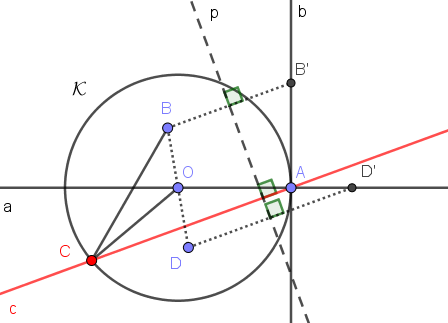
\includegraphics[width=0.6\textwidth]{images/alhazen/scimemi.png}
    \caption[Scimemijeva rešitev]{Scimemijeva rešitev Alhazenovega problema, ko točka $A$ leži na krožnici.}
    \label{fig:scimemi}
\end{figure}

\begin{trditev}
    Točka $C$ je rešitev Alhazenovega problema za točke $O, A, B$.
\end{trditev}

\opomba{Avtor je v svoje delo vključil tudi dokaz, vendar je v njem več nejasnosti, priložena skica pa je zavajajoča. Zato je tu drug, lažji dokaz \textcolor{red}{(ki sem ga iznašla sama -- a lahko pišem tko v prvi osebi?)}.}

\begin{dokaz}
    Naj bo točka $A'$ zrcalna slika točke $A$ čez pregib $p$. Zarišemo še daljici $BA'$ in $DA'$. Potem zaradi simetrije čez pregib $p$ velja $\angle BA'D = \angle B'AD' = 90^\circ$ (slika~\ref{fig:scimemi_dokaz} levo).

    Naj bo $S$ presečišče premice $CO$ z daljico $A'B$. Ker točki $P$ in $A$ ležita na krožnici $\mathcal{K}$, je trikotnik $\triangle CAO$ z vrhom v središču $O$ enakokrak. Sledi $\angle OCA = \angle CAO = \angle CA'D$. Zadnja enakost sledi iz sovršnih kotov ob točki $A$ in simetrije čez pregib $p$. Torej sta kota z vrhom v točkah $P$ in $A'$ (na sliki~\ref{fig:scimemi_dokaz} desno) izmenična, iz česar sledi $CS \parallel DA'$. Zato velja $\angle OSB = \angle DA'B = 90^\circ$.

    \begin{figure}[h]
        \centering
        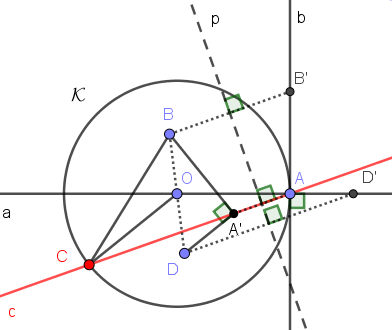
\includegraphics[width=0.47\textwidth]{images/alhazen/scimemi_dokaz1.png}
        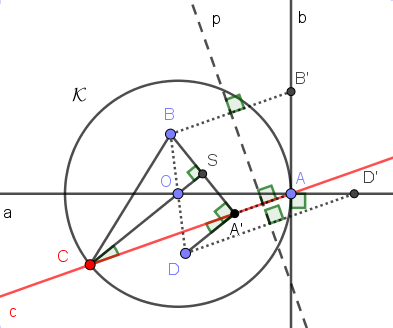
\includegraphics[width=0.47\textwidth]{images/alhazen/scimemi_dokaz2.png}
        \caption[Dokaz Scimemijeve konstrukcije]{Geometrijski dokaz Scimemijeve konstkrukcije}
        \label{fig:scimemi_dokaz}
    \end{figure}

    Trikotnika $\triangle OSB$ in $\triangle DA'B$ sta zato podobna, ker pa je $O$ središče hipotenuze večjega trikotnika, je prvi dvakrat manjši, torej $|BS| = |SA'|$.

    Zaključimo, da sta zaradi skladnih katet pravokotna trikotnika $\triangle CSB$ in $\triangle CSA'$ skladna, torej res velja $\angle SCB = \angle SCA' = \angle SCA$ oziroma daljica $OC$ res razpolavlja kot $\angle ACB$.
\end{dokaz}

\opomba{Zelo je zanimiv stranski produkt te konstrukcije -- izkaže se namreč, da točke $A, B$ in $E$ (kjer je $E$ drugo presečišče poltraka $PB$ s krožnico $\mathcal{K}$, gl.\ sliko~\ref{fig:scimemi_opomba}) ter njihove slike vse ležijo na isti krožnici! Središče te krožnice pa je presečišče poltraka $CO$ s pregibom $p$. Prav tako velja $BA' \parallel EA$ in $|BE| = |A'A|$. Dokaz za to nalogo ni ključen in ga prepuščamo bralcu.}

\begin{figure}[h]
    \centering
    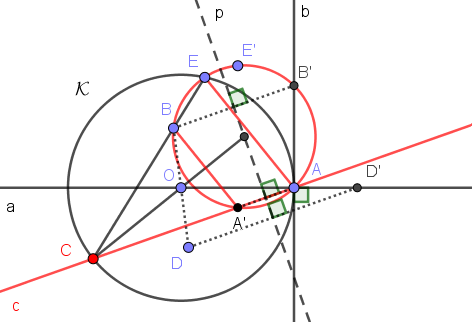
\includegraphics[width=0.6\textwidth]{images/alhazen/scimemi_stransko.png}
    \caption[Stranski produkt Scimemija]{Stranski produkti Scimemijeve konstrukcije točke $P$ (označeno z rdečo).}
    \label{fig:scimemi_opomba}
\end{figure}